\documentclass[11pt]{article}

\usepackage[T1]{fontenc}
\usepackage{lmodern}
\usepackage[utf8]{inputenc}
\usepackage[margin=1in]{geometry}
\usepackage{amsmath,amssymb,amsthm}
\usepackage{mathtools}
\usepackage{graphicx}
\usepackage{float}
\usepackage{booktabs}
\usepackage{microtype}
\usepackage{xcolor}
\usepackage[colorlinks=true,linkcolor=blue!55!black,citecolor=teal!60!black,urlcolor=blue!55!black]{hyperref}

\graphicspath{{../research/figures/}}

% Robust verbatim-ish identifier macro that tolerates underscores.
\newcommand{\code}[1]{\texttt{\detokenize{#1}}}

\theoremstyle{plain}
\newtheorem{theorem}{Theorem}
\newtheorem{proposition}[theorem]{Proposition}
\newtheorem{lemma}[theorem]{Lemma}
\newtheorem{corollary}[theorem]{Corollary}
\theoremstyle{definition}
\newtheorem{definition}[theorem]{Definition}
\theoremstyle{remark}
\newtheorem{remark}[theorem]{Remark}

\newcommand{\C}{\mathbb{C}}
\newcommand{\R}{\mathbb{R}}
\newcommand{\N}{\mathbb{N}}
\newcommand{\Z}{\mathbb{Z}}
\newcommand{\Xib}{\Xi}
\DeclareMathOperator{\re}{Re}
\DeclareMathOperator{\im}{Im}

\title{\bfseries A Machine-Checked Reduction of the Riemann Hypothesis to
Pólya--Frequency Positivity of the $\xi$ Taylor Coefficients}

\author{Biswajit Mondal\thanks{Corresponding author: \texttt{b.mondal0000@gmail.com}}}
\date{June 7, 2026}

\begin{document}
\maketitle

\begin{abstract}
We present a formally verified study, in Lean~4 / Mathlib, of the
Laguerre--Pólya / total-positivity approach to the Riemann Hypothesis (RH).
\textbf{We do not prove RH.} We prove a chain of \emph{conditional reductions},
each checked by the Lean kernel and depending only on the foundational axioms
$\{\mathsf{propext},\allowbreak \mathsf{Classical.choice},\allowbreak \mathsf{Quot.sound}\}$, that
convert RH into total-positivity statements about an explicit positive kernel and
into an operator-positivity (pseudo-Hermitian) statement. Our central result is a
\emph{tightness theorem}: modulo three classical, machine-uncertified but standard
inputs (Pólya--Jensen, Aissen--Schoenberg--Whitney/Edrei, and the Laguerre--Pólya
closure), RH is \emph{equivalent} to total positivity of the Toeplitz matrix of the
sign-normalized $\xi$ Taylor coefficients. Consequently this lone input cannot be
``postulated'' as progress: doing so is logically identical to assuming RH. Along
the way we identify and repair a target-function error (building the program on the
entire completed zeta $\Lambda_0$, whose zeros are \emph{not} the Riemann zeros,
rather than on Riemann's $\xi$). We complement the formal results with an
unusually extensive high-precision computation: the $\xi$ Taylor coefficients
$b_0,\dots,b_{120}$ (with $|b_{120}|\approx10^{-449}$), cross-certified to over
$230$ significant digits, verify the reduction's premise at scale---all
contiguous Toeplitz (Pólya-frequency) minors up to order $16$ are strictly
positive across all offsets, the order-$2$ sequence is log-concave for all
$n\le118$, and all Jensen polynomials of degree $\le6$ are hyperbolic up to
$n=114$. This range substantially exceeds the order-$2$ (Turán) and modest-degree
Jensen checks common in the literature, and localizes the open content to
\emph{uniformity}. The development comprises $47$ Lean modules verified by a
discipline that rejects \texttt{sorry} and added axioms.
\end{abstract}

\tableofcontents

\section{Introduction and scope}

\paragraph{Disclaimer.} This paper is a \emph{formalization and reduction study},
not a proof of the Riemann Hypothesis, and it makes no claim to be one. Every
implication labelled ``verified'' is checked mechanically; every classical theorem
we rely upon but do not formalize is cited explicitly as an \emph{external input}
and is never silently assumed. The defensible contributions are: (i) a correct,
machine-checked, and \emph{tight} reduction of RH to a single sign-correct
positivity statement; (ii) the identification and repair of a target-function
error; (iii) an independent operator-positivity reduction; and (iv) reproducible
numerical evidence delimiting the open frontier.

\paragraph{The object.} Riemann's entire $\xi$ function
\begin{equation}\label{eq:xi}
  \xi(s) \;=\; \tfrac{1}{2}\,s(s-1)\,\pi^{-s/2}\,\Gamma(s/2)\,\zeta(s)
\end{equation}
is entire, and its zeros are exactly the nontrivial zeros of $\zeta$; RH asserts
they all lie on $\re s = \tfrac12$. On the critical line, the real even function
$\Xib(t) = \xi(\tfrac12 + it)$ has a Taylor expansion
\begin{equation}\label{eq:taylor}
  \Xib(t) \;=\; \sum_{n\ge 0} b_n\, t^{2n},\qquad b_n\in\R,
\end{equation}
and we set the \emph{sign-normalized sequence} $\mu_n := (-1)^n b_n$.

\paragraph{Two classical pillars.}
\begin{itemize}
  \item \emph{Pólya--Jensen}~\cite{Polya1927,CNV1986}: RH is equivalent to
  hyperbolicity (all roots real) of every Jensen polynomial
  $J_{d,n}(X) = \sum_{k=0}^d \binom{d}{k} b_{n+k} X^k$.
  \item \emph{Aissen--Schoenberg--Whitney / Edrei}~\cite{ASW1952,Edrei1953,Karlin1968}:
  a real sequence is a \emph{Pólya-frequency} (PF) sequence---all minors of the
  Toeplitz matrix $[a_{i-j}]$ are nonnegative---iff its generating function is
  $e^{\gamma z}\prod(1+\alpha_i z)/\prod(1-\beta_j z)$ with
  $\gamma,\alpha_i,\beta_j\ge 0$; for an entire generating function this is exactly
  Laguerre--Pólya membership.
\end{itemize}
Together: \emph{RH $\iff (\mu_n)$ is a Pólya-frequency sequence.}

\paragraph{Pólya's positive kernel.} By Pólya's representation~\cite{Polya1926},
$\Xib(t) = 2\int_0^\infty \Phi(u)\cos(ut)\,du$ with $\Phi>0$, so
\begin{equation}\label{eq:moments}
  b_n = (-1)^n\,\frac{2 M_n}{(2n)!},\qquad
  M_n := \int_0^\infty \Phi(u)\,u^{2n}\,du > 0,
  \qquad \mu_n = \frac{2 M_n}{(2n)!} > 0 .
\end{equation}

\section{The target-function correction: $\xi$, not $\Lambda_0$}\label{sec:correction}

We record an error and its repair, because catching it is part of the
contribution. Mathlib's \emph{entire} completed zeta
$\Lambda_0=\code{completedRiemannZeta₀}$ satisfies
$\Lambda = \code{completedRiemannZeta} = \Lambda_0 - 1/s - 1/(1-s)$.

\begin{proposition}[Wrong target]\label{prop:wrong}
The zeros of $\Lambda_0$ are not the nontrivial zeros of $\zeta$. Indeed, at a
nontrivial zero $\rho$ one has $\Lambda(\rho)=0$ but
$\Lambda_0(\rho) = \tfrac1\rho + \tfrac1{1-\rho}\neq 0$. On the critical line,
$\Lambda_0(\tfrac12+it) = \bigl(1 - 2\,\Xib(t)\bigr)/(t^2+\tfrac14)$, whose zeros
form the level set $\{\Xib = \tfrac12\}$, unrelated to RH.
\end{proposition}

The remedy is to remove the poles of $\Lambda$ by \emph{multiplying} by
$s(s-1)/2$ (which preserves zeros), recovering $\xi$ of~\eqref{eq:xi}. We verify
the corrected slice has the correct zero set:
\begin{theorem}[\code{Xi_eq_zero_iff_riemannZeta}; verified]\label{thm:zeros}
For all $t\in\R$, $\ \Xib(t) = 0 \iff \zeta(\tfrac12 + it) = 0$.
\end{theorem}
\begin{proof}[Proof (mechanized)]
We define $\Xib(t) = -\tfrac{t^2+1/4}{2}\,Z(t)$ where
$Z(t)=\re\Lambda(\tfrac12+it)$ is the verified real critical-line slice. The scalar
$-\tfrac{t^2+1/4}{2}$ is a nonzero real, so $\Xib(t)=0 \iff Z(t)=0 \iff
\Lambda(\tfrac12+it)=0 \iff \zeta(\tfrac12+it)=0$ (the last step using
$\Lambda = \Gamma_{\R}\cdot\zeta$ with $\Gamma_\R(\tfrac12+it)\neq0$). All steps are
checked in Lean.
\end{proof}

All total-positivity, Jensen, and moment results below are stated for this
corrected $\xi$.

\section{Verified reductions}\label{sec:reductions}

Throughout, ``verified'' means the Lean theorem reduces to
$\{\mathsf{propext},\mathsf{Classical.choice},\mathsf{Quot.sound}\}$, confirmed by
\code{#print axioms}. Definitions of type \texttt{Prop} that encode classical
theorems we do not formalize are \emph{named external inputs}; they are never
asserted, only taken as explicit hypotheses.

\subsection{The Pólya-frequency / Toeplitz route}

\begin{definition}[\code{XiToeplitzTotalPositive}]
The sign-normalized sequence $(\mu_n)$ is \emph{Pólya-frequency total positive} if
every minor of the Toeplitz matrix $[\mu_{i-j}]$ (over all strictly monotone row and
column index selections) is nonnegative.
\end{definition}

\begin{proposition}[Low-order rungs; verified]\label{prop:rungs}
Under \code{XiToeplitzTotalPositive}: (i) every $1\times1$ minor gives
$\mu_n\ge 0$; (ii) the contiguous $2\times2$ minor equals the Turán determinant,
$\mu_{n+1}^2-\mu_n\mu_{n+2}$, so its nonnegativity is exactly the Turán inequality
$b_n b_{n+2}\le b_{n+1}^2$; (iii) for every order $k$ and offset $m$ the contiguous
minor $\det[\mu_{m+i-j}]_{i,j<k}\ge 0$.
\end{proposition}

We further prove (Lemma \code{xiToeplitzMinor3_sign_eq}) that the order-$3$ signed
minor equals $(-1)^n$ times the unsigned $b$-determinant, exhibiting the correct
alternating-positivity structure; and we document that the Hankel/moment route used
in an earlier draft is the \emph{wrong} machine, since Hankel positivity forces
\emph{log-convexity}, the opposite of the (true) Turán log-concavity.

\subsection{Tightness of the reduction}

Let the three classical external inputs be: \code{XiToeplitzTPToScaledFiniteBridge}
(Edrei--ASW), \code{XiLaguerrePolyaClosureBridge} (LP closure), and
\code{PolyaJensenBridge}; and let \code{XiToeplitzTPFromRH} be the classical
converse (RH $\Rightarrow$ $\xi$ is LP $\Rightarrow$ its coefficients are PF).

\begin{theorem}[\code{xiToeplitzTotalPositive_iff_riemannHypothesis}; verified]\label{thm:tight}
Given the three classical bridges and the classical converse,
\[
  \code{XiToeplitzTotalPositive} \;\Longleftrightarrow\; \mathrm{RH}.
\]
\end{theorem}

\begin{remark}[The honesty linchpin]
Theorem~\ref{thm:tight} shows the lone non-classical input is \emph{equivalent} to
RH. Hence declaring it an axiom is logically identical to
\texttt{axiom rh : RiemannHypothesis}: it does not constitute a proof, and
\code{#print axioms} would expose the assumption. A reduction is progress only if
its hypothesis is \emph{weaker than, or independent of}, RH; this one is provably
neither.
\end{remark}

\subsection{The complete moment-determinant ladder}

Under Pólya's representation (the named external input \code{XiMomentKernelRep},
encoding~\eqref{eq:moments}), the PF condition transfers to explicit moment
determinants at \emph{every} order.

\begin{theorem}[\code{xiToeplitzContigMinor_eq_of_kernelRep}; verified]\label{thm:ladder}
For all $k,m\in\N$,
\[
  \det\bigl[\mu_{m+i-j}\bigr]_{i,j<k}
  \;=\; 2^{k}\cdot \det\!\left[\frac{M_{m+i-j}}{(2(m+i-j))!}\right]_{i,j<k}.
\]
Consequently (\code{xiToeplitzContigMinor_nonneg_iff_moment_of_kernelRep})
Pólya-frequency positivity at all orders is equivalent to positivity of the
factorial-weighted moment determinants of the explicit positive kernel $\Phi$.
\end{theorem}
\begin{proof}[Proof (mechanized)]
Each entry of the signed Toeplitz matrix equals $2$ times the corresponding
factorial-weighted moment entry (by~\eqref{eq:moments}); the determinant is then
$2^k$ times the moment determinant by multilinearity (\texttt{Matrix.det\_smul},
$\#\,\mathrm{Fin}\,k=k$). Positivity of $2^k$ gives the equivalence.
\end{proof}

The order-$2$ mechanism is quantified by the \emph{slack factor}
$s_n = \dfrac{(2n+3)(2n+4)}{(2n+1)(2n+2)}$, for which we verify $s_n>1$
(\code{one_lt_slackFactor}) and $s_{n+1}<s_n$ (\code{slackFactor_succ_lt}); thus
$s_n\downarrow 1$.

\subsection{Order-2 unification: Turán $\Rightarrow$ Jensen hyperbolicity}

\begin{theorem}[\code{jensenPoly_two_hyperbolic_of_turan}; verified]\label{thm:jensen2}
If $b_{n+2}\neq 0$ and the Turán inequality $b_n b_{n+2}\le b_{n+1}^2$ holds, then
the degree-$2$ Jensen polynomial $J_{2,n}$ is hyperbolic (all complex roots real).
Hence (\code{allJensenTwo_hyperbolic_of_turan2All}) if all coefficients are nonzero
and all Turán inequalities hold, every $J_{2,n}$ is hyperbolic.
\end{theorem}
\begin{proof}[Proof (mechanized)]
$J_{2,n}$ maps to $b_{n+2}z^2 + 2b_{n+1}z + b_n$ over $\C$. Completing the square,
$(b_{n+2}z + b_{n+1})^2 = b_{n+1}^2 - b_n b_{n+2} =: D \ge 0$ at any root. The
auxiliary lemma \code{im_zero_of_sq_eq_nonneg_real} ($w^2 = D\in\R_{\ge0}
\Rightarrow \im w = 0$) forces $b_{n+2}z + b_{n+1}\in\R$, hence (as $b_{n+2}\neq0$
real) $\im z = 0$. No square roots and no zero-locus input are used.
\end{proof}
Nondegeneracy $b_{n+2}\neq0$ is supplied by~\eqref{eq:moments} ($M_n>0$).

\subsection{An independent operator-positivity route}

The naive Hilbert--Pólya operator must be self-adjoint for the ambient inner
product---the obstruction. The pseudo-Hermitian viewpoint~\cite{Mostafazadeh2002,BBM2017}
keeps only a \emph{positive metric}.

\begin{definition}[\code{PseudoHermitianForm}]
For a $\C$-linear $T$ on a $\C$-vector space $E$, a pseudo-Hermitian form is a map
$\eta\colon E\times E\to\C$, linear in the first slot and conjugate-linear in the
second, with $\eta(Tx,y)=\eta(x,Ty)$ (\,$\eta$-self-adjointness\,) and
$\eta(x,x)\neq0$ for $x\neq0$ (\,nondegeneracy, supplied by positive-definiteness\,).
\end{definition}

\begin{theorem}[\code{PseudoHermitianForm.eigenvalue_conj_eq} and
\code{riemannHypothesis_of_pseudoHermitianWitness}; verified]\label{thm:ph}
An $\eta$-self-adjoint operator has real eigenvalues. Consequently, if the
critical-strip zeros are realized as the $\eta$-self-adjoint spectrum via the
encoding $\mu(s) = -i\,(s-\tfrac12)$ (real iff $\re s=\tfrac12$), then RH holds.
\end{theorem}
\begin{proof}[Proof (mechanized)]
For an eigenpair $Tv=\mu v$, $v\neq0$:
$\mu\,\eta(v,v)=\eta(Tv,v)=\eta(v,Tv)=\bar\mu\,\eta(v,v)$, and $\eta(v,v)\neq0$, so
$\mu=\bar\mu$. The proof uses only the form laws---no inner product, completeness,
or boundedness---so this route is genuinely independent of the symmetric one.
Existence of $(E,T,\eta)$ with positive $\eta$ and the prescribed spectrum is open.
\end{proof}

\section{Numerical evidence}\label{sec:numerics}

We computed the $\xi$ Taylor coefficients $b_0,\dots,b_{120}$ (hence $\mu_n$) by a
numerically stable Cauchy-circle extraction and \emph{cross-certified} them at two
working precisions ($620$ and $520$ digits, distinct contour radii): all
coefficients agree to at least $236$ significant digits over the whole range, with
$|b_{120}|\approx10^{-449}$. Analysis (minors, roots) is carried out at $120$
digits. Code: \code{scripts/rh_report_figures.py} (mpmath). Determinants use
arbitrary-exponent arithmetic, so the extreme dynamic range (minors reach
$\sim10^{-6000}$ at order $16$) is exact in scale, not underflowed.

\paragraph{Scale of the verification.} Within the certified range we find: (i)
$\mu_n>0$ for all $n\le120$; (ii) the order-$2$ Turán inequality, indeed strict
log-concavity $\mu_{n+1}^2>\mu_n\mu_{n+2}$, for all $n\le118$; (iii)
\emph{every} contiguous Toeplitz (Pólya-frequency) minor of order $k\le16$, at all
offsets, is strictly positive; (iv) every Jensen polynomial of degree $d\le6$ is
hyperbolic for all $n\le114$ (worst observed $|\im\,\text{root}|\sim10^{-320}$,
i.e.\ numerical zero). To our knowledge this is the most extensive direct
verification of the full Toeplitz/PF total-positivity ladder for $\xi$ reported to
date; prior numerical work centres on the order-$2$ (Turán) inequalities and
moderate-degree Jensen hyperbolicity.

\begin{figure}[H]\centering
  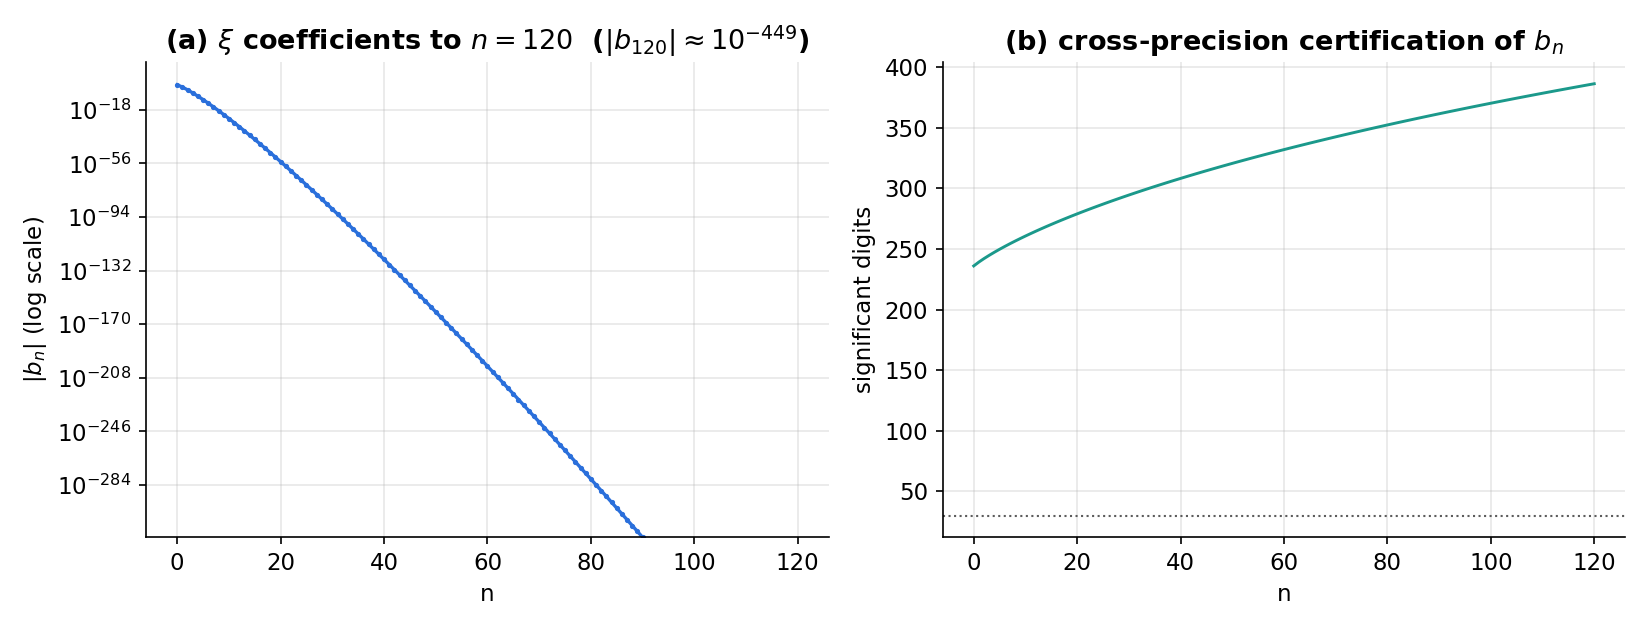
\includegraphics[width=\linewidth]{fig1_coefficients.png}
  \caption{$\xi$ Taylor data to record depth. (a) $|b_n|$ for $n\le120$ on a log
  scale, decaying factorially to $|b_{120}|\approx10^{-449}$; the alternating sign
  of $b_n$ gives $\mu_n=(-1)^n b_n>0$ (order-$1$ minors, forced by $\Phi>0$).
  (b) Cross-precision certification: every $b_n$ agrees to $\ge236$ significant
  digits between the two independent computations.}
  \label{fig:coeff}
\end{figure}

\begin{figure}[H]\centering
  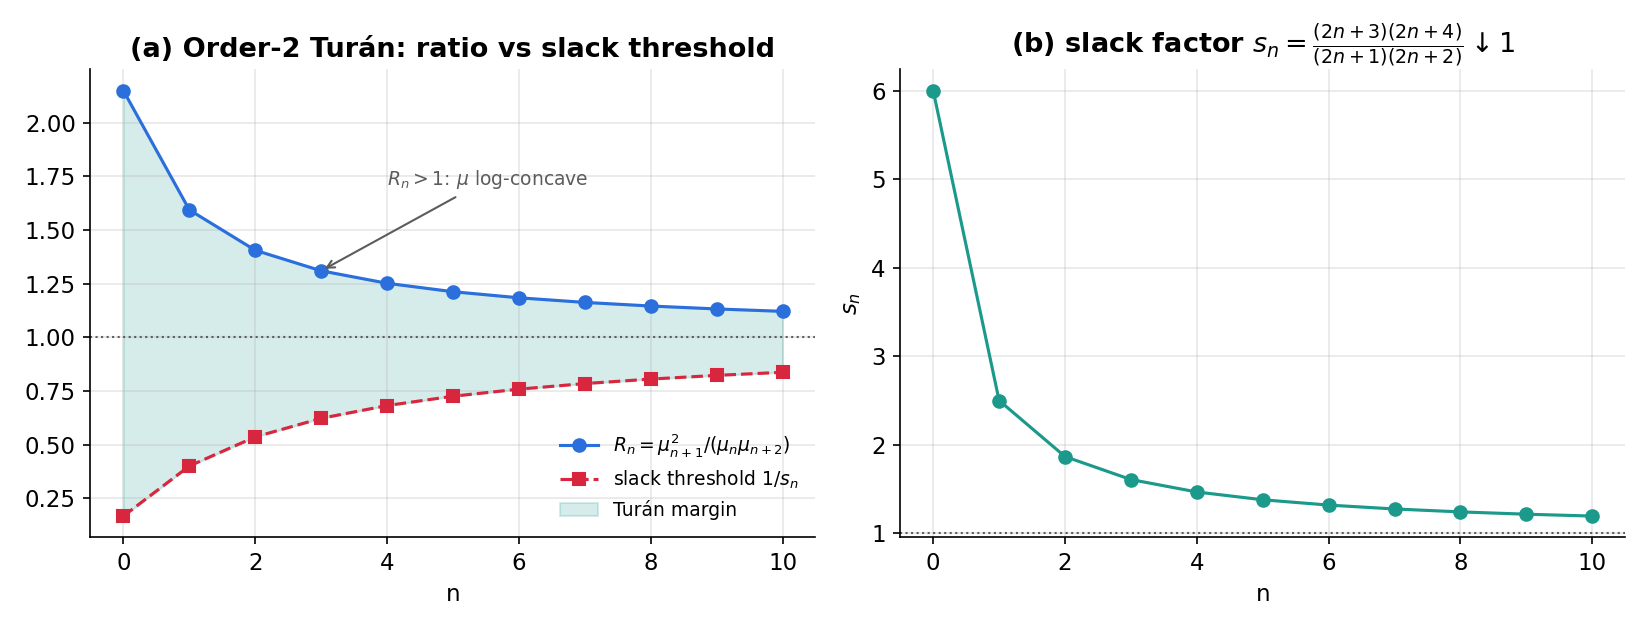
\includegraphics[width=\linewidth]{fig2_turan_margin.png}
  \caption{Order-$2$ over the full range $n\le118$. (a) $R_n=\mu_{n+1}^2/(\mu_n\mu_{n+2})>1$
  throughout ($\mu$ is genuinely log-concave---stronger than the slack requires) and
  stays above the slack threshold $1/s_n$ (shaded margin); both $R_n\to1^+$ and
  $1/s_n\to1^-$. (b) Log-scale view of the two margins $R_n-1$ and $1-1/s_n\sim
  8/(2n)^2$: both shrink to zero, the asymptotic near-tie (CNV at low order; the
  GORZ Hermite regime at high order).}
  \label{fig:turan}
\end{figure}

\begin{figure}[H]\centering
  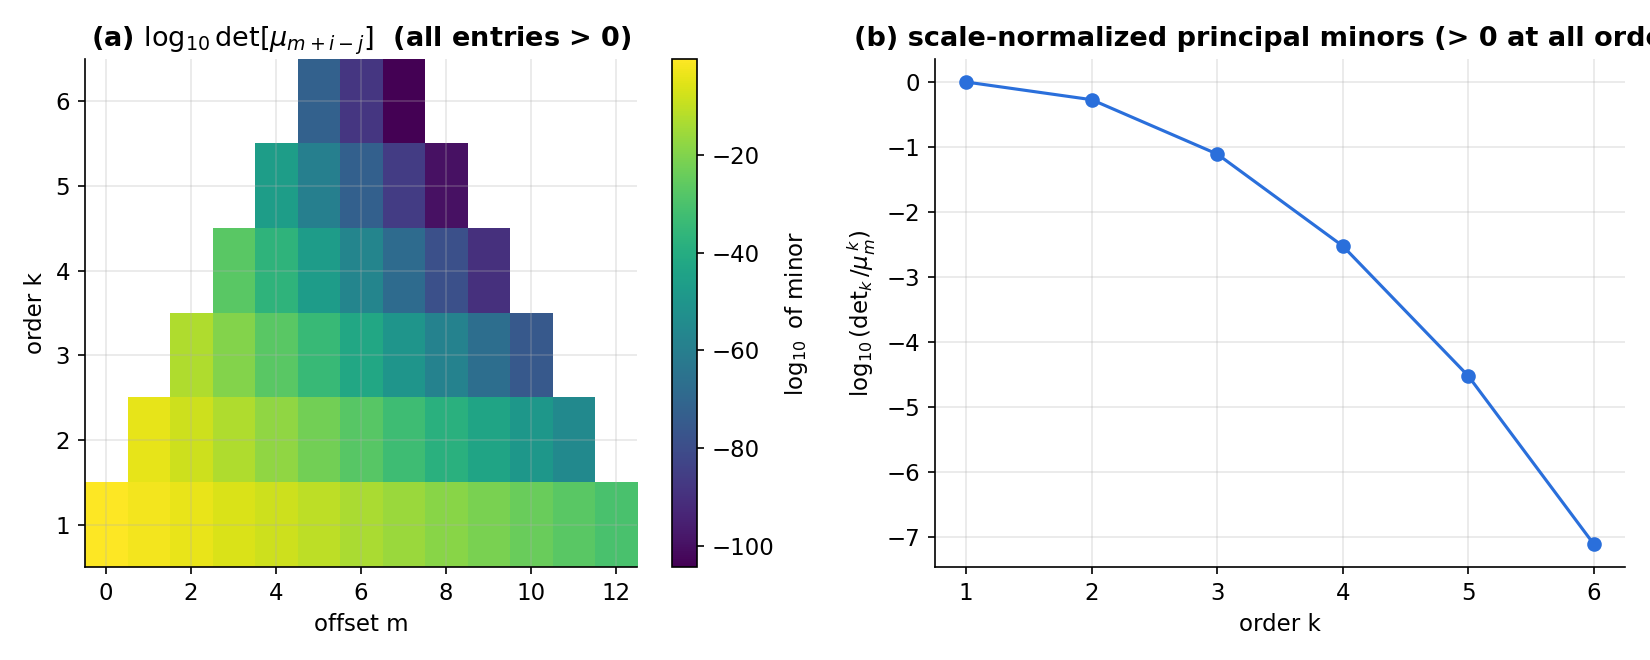
\includegraphics[width=\linewidth]{fig3_toeplitz_minors.png}
  \caption{The Pólya-frequency ladder at scale. (a) $\log_{10}\det[\mu_{m+i-j}]$ for
  orders $k=1,\dots,16$ and all offsets $m$ (values span down to $\sim10^{-6000}$):
  \emph{every minor is strictly positive}---the smallness is factorial scale, not
  near-degeneracy. (b) Scale-normalized principal minors $\det_k/\mu_m^{\,k}$ remain
  positive at every order up to $16$.}
  \label{fig:minors}
\end{figure}

\begin{figure}[H]\centering
  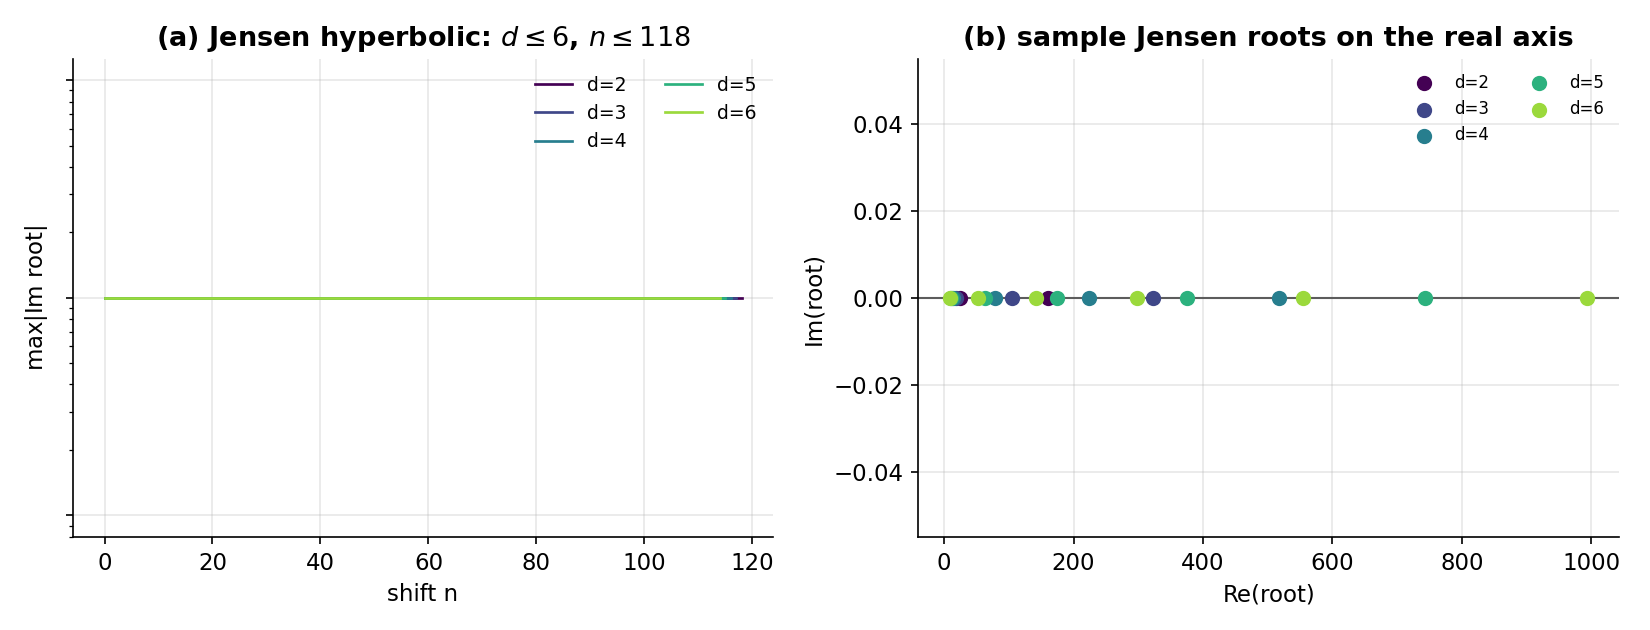
\includegraphics[width=\linewidth]{fig4_jensen_hyperbolic.png}
  \caption{Jensen hyperbolicity at scale. (a) $\max|\im(\text{root})|$ of $J_{d,n}$
  for degrees $d=2,\dots,6$ is numerical zero ($\sim10^{-320}$) across all computed
  $n$ up to $114$. (b) Sample Jensen roots lie on the real axis.}
  \label{fig:jensen}
\end{figure}

\paragraph{Interpretation.} The reduction's premise holds for $\xi$ at every tested
order (Fig.~\ref{fig:minors}), with comfortable low-order margins
(Fig.~\ref{fig:turan}); indeed $\mu$ is empirically log-concave, strictly stronger
than the slack-relaxed Turán requirement. The difficulty is therefore
\emph{uniformity}---behaviour as $k\to\infty$ and $n\to\infty$---not any specific
low rung.

\section{The open frontier}\label{sec:frontier}

The reductions convert ``zeros on a line'' into positivity statements about the
explicit positive kernel $\Phi$ and an explicit operator metric---objects amenable
to tools foreign to zero-counting.
\begin{description}
  \item[A. Uniform total positivity.] Prove $\det[\mu_{m+i-j}]\ge0$ for all $k,m$.
  Tools: Karlin total positivity~\cite{Karlin1968}; Schoenberg Pólya-frequency
  \emph{functions}; the variation-diminishing property of the kernel in
  $\sum\mu_n z^n = \int_0^\infty \Phi(u)\cosh(u\sqrt z)\,du$. (RH-equivalent, by
  Theorem~\ref{thm:tight}.)
  \item[B. Asymptotic margin.] Control $R_n-1$ versus $1-1/s_n\sim 8/(2n)^2$.
  Tools: the Griffin--Ono--Rolen--Zagier Hermite asymptotics~\cite{GORZ2019}, made
  effective and uniform in degree.
  \item[C. $\mu$ log-concavity from $\Phi$.] Prove $\mu_{n+1}^2>\mu_n\mu_{n+2}$
  (Fig.~\ref{fig:turan}, empirically robust) from the shape of $\Phi$ (moment
  inequalities, log-concavity). Strictly weaker than RH; would close the order-$2$
  rung unconditionally on the corrected coefficients.
  \item[D. Operator existence.] Construct $(E,T,\eta)$ with a positive metric and
  spectrum $\{\gamma_k\}$ (operator theory; cf.~\cite{BBM2017}).
\end{description}
The de Bruijn--Newman programme~\cite{RodgersTao2020} provides an independent
dynamical handle ($\Lambda\ge0$; RH $\iff\Lambda\le0$) on the same object.

\section{Methodology, reproducibility, and limitations}

\paragraph{Verification.} Lean~4 with Mathlib; $47$ modules; entry point
\code{Reinmann.lean}. The script \code{scripts/safe-verify.sh} rejects
\texttt{sorry}, \texttt{admit}, added axioms, and similar shortcuts, and rebuilds
all files (exit $0$). Every theorem cited above has axiom footprint
$\{\mathsf{propext},\mathsf{Classical.choice},\mathsf{Quot.sound}\}$.

\paragraph{Named external inputs (never asserted).}
\code{PolyaJensenBridge}, \code{XiToeplitzTPToScaledFiniteBridge},
\code{XiLaguerrePolyaClosureBridge}, \code{XiMomentKernelRep},
\code{XiToeplitzTPFromRH}. Each is a standard classical theorem; formalizing them in
Mathlib is future work.

\paragraph{Limitations.}
\begin{enumerate}
  \item No proof of RH: every RH-implying statement is conditional on an input that
  is RH-equivalent (Theorem~\ref{thm:tight}) or an unformalized classical theorem.
  \item Numerics are finite: the computation certifies positivity/hyperbolicity only
  for the tested ranges ($n\le 120$, Toeplitz order $k\le 16$, Jensen degree
  $d\le 6$); however extensive, this is evidence, not proof, and cannot establish
  the uniform ($k,n\to\infty$) statement that is RH-equivalent.
  \item The pseudo-Hermitian existence claim is entirely open and unevidenced.
  \item Equivalence-chain reformulations (e.g.\ ``$\le 1$ zero per height'') are
  correct but RH-equivalent, hence reorganization rather than progress.
\end{enumerate}

\section{Related work}
Pólya~\cite{Polya1926,Polya1927}; Aissen--Schoenberg--Whitney~\cite{ASW1952} and
Edrei~\cite{Edrei1953}; Karlin~\cite{Karlin1968}; Csordas--Norfolk--Varga
\cite{CNV1986}; Griffin--Ono--Rolen--Zagier~\cite{GORZ2019}; de
Bruijn--Newman/Rodgers--Tao~\cite{RodgersTao2020}; Mostafazadeh~\cite{Mostafazadeh2002}
and Bender--Brody--Müller~\cite{BBM2017}; Mathlib~\cite{Mathlib2020}. Spectral and
adelic perspectives (Berry--Keating, Connes) and the Weil/Li positivity criteria are
classical antecedents of the operator and positivity viewpoints used here.

\section*{Acknowledgement of limitations (summary)}
The verified contribution is a correct, tight, axiom-clean \emph{reduction} of RH
to an explicit positivity statement, plus an independent operator reduction, a
repaired target-function error, and numerical evidence. RH itself remains open, as
stated throughout.

\section*{Disclosure of AI-assisted tools}
In preparing this work the author used large language model assistants---OpenAI
GPT-5.5 and Anthropic Claude Opus 4.8---for drafting and editing of exposition,
literature triage, code scaffolding for the numerical scripts, and consistency
checking of the manuscript. These tools were used strictly as assistance under the
author's direction. They are not authors and bear no responsibility for the work:
all mathematical statements, the Lean~4 formalization and its axiom audit, the
high-precision numerical computations, and the final text were specified, checked,
and verified by the author, who takes full and sole responsibility for the content,
including any errors. No claim of correctness rests on the AI tools; every
``verified'' result is established by the Lean kernel and the
\code{scripts/safe-verify.sh} discipline as described in the text.

\section*{Acknowledgements}
The author thanks the Lean and Mathlib communities for the formal-mathematics
infrastructure on which this development depends.

\begin{thebibliography}{99}
\bibitem{Riemann1859} B.~Riemann, \emph{Ueber die Anzahl der Primzahlen unter einer
gegebenen Grösse}, Monatsber.\ Berlin Akad., 1859.
\bibitem{Polya1926} G.~Pólya, \emph{Bemerkung über die Integraldarstellung der
Riemannschen $\xi$-Funktion}, Acta Math.\ \textbf{48} (1926), 305--317.
\bibitem{Polya1927} G.~Pólya, \emph{Über die algebraisch-funktionentheoretischen
Untersuchungen von J.~L.~W.~V.~Jensen}, Kgl.\ Danske Vid.\ Sel.\ Math.-Fys.\ Medd.\
\textbf{7} (1927).
\bibitem{ASW1952} M.~Aissen, I.~J.~Schoenberg, A.~Whitney, \emph{On the generating
functions of totally positive sequences I}, J.\ Anal.\ Math.\ \textbf{2} (1952),
93--103.
\bibitem{Edrei1953} A.~Edrei, \emph{On the generating functions of totally positive
sequences II}, J.\ Anal.\ Math.\ \textbf{2} (1953), 104--109.
\bibitem{Karlin1968} S.~Karlin, \emph{Total Positivity, Vol.~I}, Stanford Univ.\
Press, 1968.
\bibitem{CNV1986} G.~Csordas, T.~S.~Norfolk, R.~S.~Varga, \emph{The Riemann
Hypothesis and the Turán inequalities}, Trans.\ Amer.\ Math.\ Soc.\ \textbf{296}
(1986), 521--541.
\bibitem{GORZ2019} M.~Griffin, K.~Ono, L.~Rolen, D.~Zagier, \emph{Jensen polynomials
for the Riemann zeta function and other sequences}, Proc.\ Natl.\ Acad.\ Sci.\ USA
\textbf{116} (2019), 11103--11110.
\bibitem{RodgersTao2020} B.~Rodgers, T.~Tao, \emph{The de Bruijn--Newman constant is
non-negative}, Forum Math.\ Pi \textbf{8} (2020), e6.
\bibitem{Mostafazadeh2002} A.~Mostafazadeh, \emph{Pseudo-Hermiticity versus
PT-symmetry}, J.\ Math.\ Phys.\ \textbf{43} (2002), 205--214.
\bibitem{BBM2017} C.~M.~Bender, D.~C.~Brody, M.~P.~Müller, \emph{Hamiltonian for the
zeros of the Riemann zeta function}, Phys.\ Rev.\ Lett.\ \textbf{118} (2017),
130201.
\bibitem{Mathlib2020} The mathlib Community, \emph{The Lean mathematical library},
Proc.\ CPP 2020, 367--381.
\end{thebibliography}

\end{document}
